\documentclass[12pt]{article}
\usepackage[utf8]{inputenc}
\usepackage{tikz}
\usetikzlibrary{positioning, shapes.geometric, arrows.meta, shadows}
\usepackage{geometry}
\geometry{a4paper, margin=1in}
\usepackage{sectsty}
\sectionfont{\large\bfseries}
\usepackage{enumitem}
\usepackage{amsmath}
\usepackage{booktabs}
\usepackage{longtable}
\usepackage{array}
\usepackage{verbatim}
\usepackage[unicode]{hyperref}

\title{Comprehensive Swarm Drone System: Data Flows and Navigation in Radio Electronic Jamming Conditions}
\author{}
\date{June 15, 2025}

\begin{document}

\maketitle

\tableofcontents
\newpage

% PART I: DATA FLOWS IN DRONE SWARM
\section*{Part I: Data Flows in Drone Swarm}
\addcontentsline{toc}{section}{Part I: Data Flows in Drone Swarm}

\section{System Overview}

The developed system represents a swarm of 100 autonomous drones organized in a three-level hierarchical structure. The main objective is conducting reconnaissance, mapping, and data transmission in conditions of radio frequency communication absence, with minimal vulnerability to detection. To ensure effective interaction between levels, laser and infrared communication technologies with line-of-sight priority are used.

Each level performs specialized functions:
\begin{itemize}
    \item \textbf{Level 1 (Command)} --- high-power drones with LIDAR sensors and base communication capabilities.
    \item \textbf{Level 2 (Relay)} --- intermediate relay drones and navigation beacons.
    \item \textbf{Level 3 (Worker)} --- small drones responsible for ground reconnaissance.
\end{itemize}

The system is also capable of integrating with external FPV strike drones, to which reconnaissance data is promptly transmitted for subsequent target engagement decisions.

\section{Integration with NATO and Ukraine Systems}

To ensure compatibility with existing NATO and AFU (Armed Forces of Ukraine) architecture, the swarm system must support the following interfaces, protocols, and standards:

\subsection{NATO Tactical and Strategic Systems}
\begin{itemize}
    \item \textbf{Link 16} --- tactical digital data transmission network. Integration through gateways with IP tunneling or JREAP support.
    \item \textbf{JREAP-C} --- Link 16 extension over IP. Capability to relay intelligence data from command drones (level 1) through ground station.
    \item \textbf{STANAG 4586} --- UAV interaction standard. Support for command and telemetry exchange interface.
    \item \textbf{STANAG 4609 / 4545} --- video and intelligence data formats (ISR). Used for transmitting streams from cameras and lidars.
    \item \textbf{FMN (Federated Mission Networking)} --- NATO common mission network. Support for federated routing and metadata.
    \item \textbf{MAJIIC II / MAJIIC III} --- multinational intelligence exchange architecture. Capability for automatic routing of target coordinates and events.
\end{itemize}

\subsection{AFU Systems and Ukrainian Combat Interfaces}
\begin{itemize}
    \item \textbf{Delta} --- Ukrainian-made C4ISR platform. Requires REST API, JSON-compatible, with target coordinates and map transmission.
    \item \textbf{Kropyva} --- digital artillery control system. Integration possible through target coordinate export in UTM/LL format.
    \item \textbf{GIS Arta / ArtOS} --- fire control geoinformation systems. Support for intelligence data transmission via UDP/TCP through API gateways.
    \item \textbf{REDCON / BMS platforms} --- tactical control interfaces. Support for interaction through MQTT/BROKER layers and secure API.
    \item \textbf{New generation FPV controllers} --- interaction through mobile command stations or swarm hubs transmitting real-time targeting.
\end{itemize}

\textbf{Note:} All interfaces must be implemented through translators, gateways, or containerized API proxies deployed on command drones or ground stations. Priority --- compatibility, scalability, and security.

\section{Gateway Architecture and API Interaction}
\subsection{Gateway Architecture Diagram}
\begin{center}
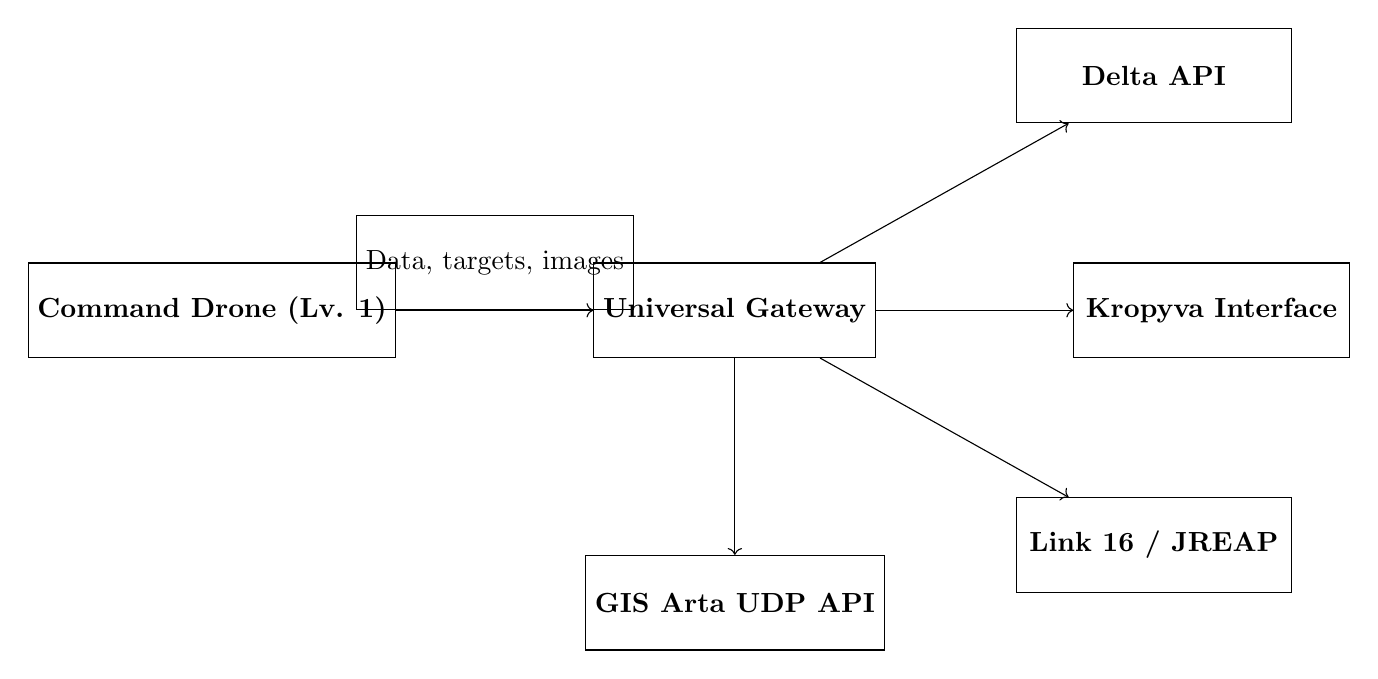
\begin{tikzpicture}[node distance=2.5cm, every node/.style={draw, align=center, minimum width=3.5cm, minimum height=1.2cm}]
\node (drone) {\textbf{Command Drone (Lv. 1)}};
\node[right=of drone] (gateway) {\textbf{Universal Gateway}};
\node[above right=of gateway] (delta) {\textbf{Delta API}};
\node[right=of gateway] (kropyva) {\textbf{Kropyva Interface}};
\node[below right=of gateway] (link16) {\textbf{Link 16 / JREAP}};
\node[below=of gateway] (gisarta) {\textbf{GIS Arta UDP API}};
\draw[->] (drone) -- node[above] {Data, targets, images} (gateway);
\draw[->] (gateway) -- (delta);
\draw[->] (gateway) -- (kropyva);
\draw[->] (gateway) -- (link16);
\draw[->] (gateway) -- (gisarta);
\end{tikzpicture}
\end{center}

\subsection{API Request Examples}

\paragraph{Delta API --- JSON REST example:}
\begin{verbatim}
POST /api/v1/targets HTTP/1.1
Host: delta.local
Content-Type: application/json
Authorization: Bearer <token>

{
  "target_id": "drone_4231",
  "lat": 48.3794,
  "lon": 31.1656,
  "type": "vehicle",
  "confidence": 0.92,
  "source": "swarm_uav"
}
\end{verbatim}

\paragraph{Kropyva --- coordinate transmission in UTM format:}
\begin{verbatim}
{
  "utm_zone": "36N",
  "easting": 345210,
  "northing": 5032123,
  "target_type": "infantry",
  "accuracy_m": 10
}
\end{verbatim}

\paragraph{GIS Arta --- UDP target transmission packet:}
\begin{verbatim}
HEADER: ARTOS
PAYLOAD:
{
  "id": "obj_101",
  "coordinates": [48.40, 31.12],
  "classification": "tank",
  "priority": 1
}
\end{verbatim}

\paragraph{Link 16 / JREAP-C --- target coordinate conversion:}
\begin{verbatim}
[TargetReport]
ID = 9032
Latitude = 48.3794
Longitude = 31.1656
TrackQuality = 5
Classification = GroundVehicle
TimeStamp = UTC2025-06-15T12:05:32Z
\end{verbatim}

\newpage

% PART II: NAVIGATION TECHNOLOGIES
\section*{Part II: Navigation Technologies in RF Jamming Environments}
\addcontentsline{toc}{section}{Part II: Navigation Technologies in RF Jamming Environments}

\section{Introduction}
Swarm drone UAVs operating in RF jamming environments require robust navigation technologies to maintain coordination and functionality, as traditional RF-based systems like GPS are unreliable. This document details nine key technologies used for navigation in such conditions: Inertial Navigation Systems (INS), Visual-Inertial Odometry (VIO), Ultra-Wideband (UWB) Localization, LiDAR-Based SLAM, Optical Flow Sensors, Acoustic/Ultrasonic Sensing, Edge AI and Onboard Processing, Magnetic Navigation, and Decentralized Swarm Algorithms. These technologies are compared in a table, and their integration is visualized in an action diagram.

\section{Navigation Technologies}
The following technologies enable swarm drone navigation in RF jamming environments:

\begin{itemize}[label=$\bullet$]
    \item \textbf{Inertial Navigation Systems (INS):} Combines accelerometers, gyroscopes, and magnetometers to estimate position, orientation, and velocity without external signals. INS is jam-resistant but may drift over time, requiring periodic corrections.
    \item \textbf{Visual-Inertial Odometry (VIO):} Uses cameras and inertial sensors to track motion by analyzing visual features. VIO fuses image data with inertial measurements for precise navigation in GPS-denied environments.
    \item \textbf{Ultra-Wideband (UWB) Localization:} Employs short-range, high-bandwidth pulses for precise relative positioning among drones. UWB resists RF jamming due to its wide frequency spectrum and low power requirements.
    \item \textbf{LiDAR-Based SLAM:} Uses laser scanners for Simultaneous Localization and Mapping (SLAM) to create 3D maps and track position. Effective in complex, GPS-denied areas and immune to RF interference.
    \item \textbf{Optical Flow Sensors:} Analyzes visual patterns on the ground to estimate velocity, aiding stable flight and hover control at low altitudes in jamming environments.
    \item \textbf{Acoustic/Ultrasonic Sensing:} Detects obstacles or relative drone positions using sound waves, suitable for short-range coordination and collision avoidance.
    \item \textbf{Edge AI and Onboard Processing:} Processes sensor data locally to enable autonomous decision-making and swarm coordination without external communication.
    \item \textbf{Magnetic Navigation:} Uses Earth's magnetic field for orientation, serving as a fallback when other systems are compromised.
    \item \textbf{Decentralized Swarm Algorithms:} Enables drones to coordinate using local sensor data and peer-to-peer communication (e.g., via UWB or optical signals), reducing reliance on centralized RF control.
\end{itemize}

These technologies are often fused using sensor fusion algorithms (e.g., Kalman filters) to enhance accuracy and robustness, with redundancy to counter jamming effects.

\section{Comparison of Navigation Technologies}
The table below compares the navigation technologies based on their primary use, frequency band, and technical capabilities, providing a competitive overview.

\begin{longtable}{|>{\raggedright\arraybackslash}p{3cm}|>{\raggedright\arraybackslash}p{3.5cm}|>{\raggedright\arraybackslash}p{3cm}|>{\raggedright\arraybackslash}p{6cm}|}
    \hline
    \textbf{Technology} & \textbf{Primary Use} & \textbf{Frequency Band} & \textbf{Technical Capabilities} \\
    \hline
    \endfirsthead
    \hline
    \textbf{Technology} & \textbf{Primary Use} & \textbf{Frequency Band} & \textbf{Technical Capabilities} \\
    \hline
    \endhead
    \hline
    \endfoot
    \hline
    \endlastfoot
    Inertial Navigation Systems (INS) & Position, orientation, and velocity estimation & None (sensor-based) & High accuracy over short durations (0.1--1 m error after 1 min); prone to drift over time; requires periodic correction; lightweight (50--500 g). \\
    \hline
    Visual-Inertial Odometry (VIO) & Motion tracking and localization & None (camera-based) & High precision (0.1--0.5 m) in well-lit, textured environments; computationally intensive; limited by camera range (5--50 m); robust to RF jamming. \\
    \hline
    Ultra-Wideband (UWB) Localization & Relative positioning among drones & 3.1--10.6 GHz & Sub-meter accuracy (10--30 cm); short range (10--100 m); low power (0.1--1 W); resistant to multipath and jamming; requires line-of-sight. \\
    \hline
    LiDAR-Based SLAM & 3D mapping and localization & None (laser-based) & High accuracy (1--10 cm); effective in complex environments; long range (10--200 m); high computational load; costly and heavy (0.5--5 kg). \\
    \hline
    Optical Flow Sensors & Velocity estimation and hover control & None (camera-based) & Good for low-altitude flight (0.5--10 m); accuracy of 1--5 cm/s; sensitive to lighting and surface texture; lightweight (10--100 g). \\
    \hline
    Acoustic/Ultrasonic Sensing & Obstacle detection and short-range coordination & 20--40 kHz & Short range (1--10 m); accuracy of 1--5 cm; unaffected by RF jamming; sensitive to environmental noise and wind. \\
    \hline
    Edge AI and Onboard Processing & Autonomous decision-making and sensor fusion & None (software-based) & Enables real-time processing; supports complex algorithms (e.g., Kalman filters); requires high computational power (1--10 W); scalable for swarm coordination. \\
    \hline
    Magnetic Navigation & Orientation estimation & None (magnetic-based) & Low accuracy (1--5° error); long-range applicability; immune to RF jamming; susceptible to magnetic interference; lightweight (10--50 g). \\
    \hline
    Decentralized Swarm Algorithms & Swarm coordination and navigation & Varies (e.g., UWB, optical) & Enables peer-to-peer coordination; fault-tolerant; reduces reliance on centralized control; depends on local sensor range and communication reliability. \\
    \hline
    \caption{Comparison of navigation technologies for swarm drone UAVs in RF jamming environments.}
    \label{tab:nav_tech}
\end{longtable}

\section{Action Diagram}
The action diagram below illustrates how a swarm drone integrates these navigation technologies. Sensors (INS, VIO, UWB, LiDAR, Optical Flow, Acoustic, Magnetic) provide raw data to Edge AI for fusion and processing. Decentralized Swarm Algorithms enable coordination with other drones, with feedback to Edge AI for iterative refinement. The drone uses the resulting commands for navigation and swarm behavior in an RF jamming environment.

\begin{figure}[h]
    \centering
    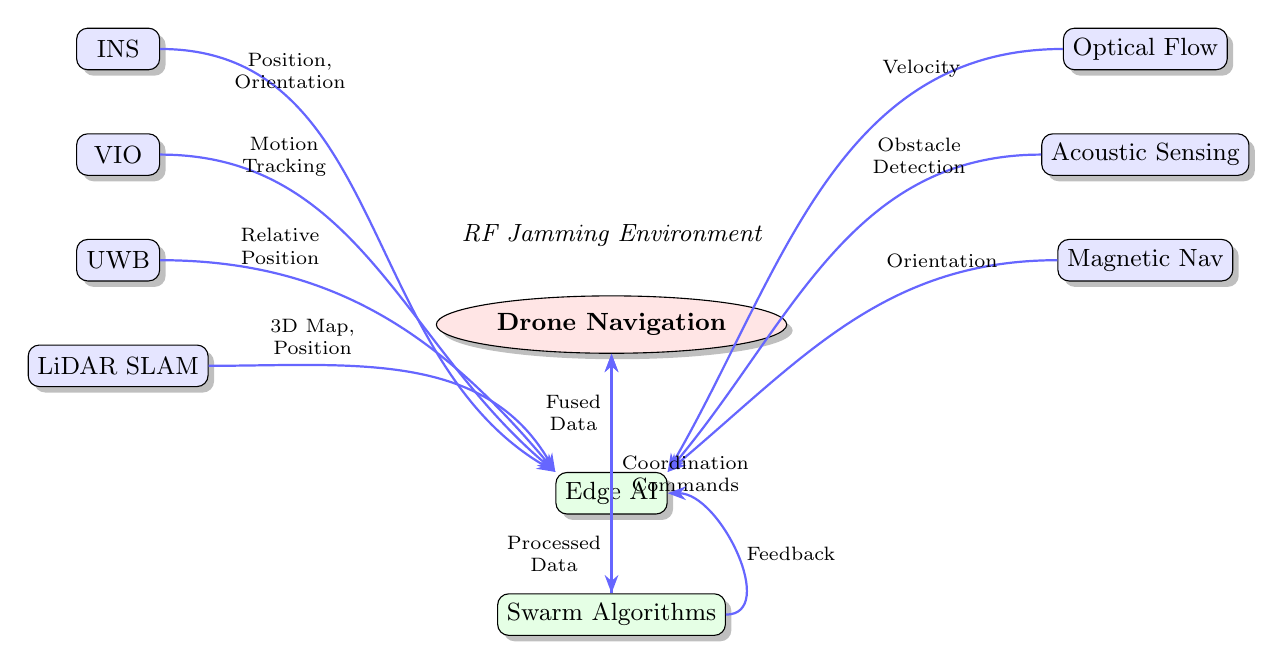
\begin{tikzpicture}[
        box/.style={rectangle, draw, rounded corners, minimum height=1.5em, minimum width=3em, text centered, font=\small, fill=blue!10, drop shadow},
        central/.style={ellipse, draw, minimum height=2em, minimum width=6em, text centered, font=\small\bfseries, fill=red!10, drop shadow},
        arrow/.style={-Stealth, thick, draw=blue!60},
        process/.style={rectangle, draw, rounded corners, minimum height=1.5em, minimum width=4em, text centered, font=\small, fill=green!10, drop shadow},
        node distance=1.5cm and 2.5cm
    ]
    
    % Central drone node
    \node[central] (drone) {Drone Navigation};
    
    % Sensor nodes (left side)
    \node[box, left=3.5cm of drone, yshift=3.5cm] (ins) {INS};
    \node[box, below=0.8cm of ins] (vio) {VIO};
    \node[box, below=0.8cm of vio] (uwb) {UWB};
    \node[box, below=0.8cm of uwb] (lidar) {LiDAR SLAM};
    
    % Sensor nodes (right side)
    \node[box, right=3.5cm of drone, yshift=3.5cm] (optical) {Optical Flow};
    \node[box, below=0.8cm of optical] (acoustic) {Acoustic Sensing};
    \node[box, below=0.8cm of acoustic] (magnetic) {Magnetic Nav};
    
    % Processing nodes
    \node[process, below=1.5cm of drone] (ai) {Edge AI};
    \node[process, below=1cm of ai] (swarm) {Swarm Algorithms};
    
    % Arrows from sensors to Edge AI (curved for clarity)
    \draw[arrow] (ins.east) to[out=0,in=150] node[near start, above, font=\scriptsize, align=center] {Position,\\Orientation} (ai.north west);
    \draw[arrow] (vio.east) to[out=0,in=140] node[near start, above, font=\scriptsize, align=center] {Motion\\Tracking} (ai.north west);
    \draw[arrow] (uwb.east) to[out=0,in=130] node[near start, above, font=\scriptsize, align=center] {Relative\\Position} (ai.north west);
    \draw[arrow] (lidar.east) to[out=0,in=120] node[near start, above, font=\scriptsize, align=center] {3D Map,\\Position} (ai.north west);
    \draw[arrow] (optical.west) to[out=180,in=60] node[near start, above, font=\scriptsize, align=center] {Velocity} (ai.north east);
    \draw[arrow] (acoustic.west) to[out=180,in=50] node[near start, above, font=\scriptsize, align=center] {Obstacle\\Detection} (ai.north east);
    \draw[arrow] (magnetic.west) to[out=180,in=40] node[near start, above, font=\scriptsize, align=center] {Orientation} (ai.north east);
    
    % Arrows from Edge AI to Drone and Swarm Algorithms
    \draw[arrow] (ai.north) -- node[midway, left, font=\scriptsize, align=center] {Fused\\Data} (drone.south);
    \draw[arrow] (ai.south) -- node[midway, left, font=\scriptsize, align=center] {Processed\\Data} (swarm.north);
    \draw[arrow] (swarm.north) -- node[midway, right, font=\scriptsize, align=center] {Coordination\\Commands} (drone.south);
    
    % Feedback loop (cleaner path)
    \draw[arrow] (swarm.east) to[out=0,in=0] node[midway, right, font=\scriptsize] {Feedback} (ai.east);
    
    % Environment label
    \node[above=0.5cm of drone, font=\small\itshape] {RF Jamming Environment};
    
    \end{tikzpicture}
    \caption{Action diagram showing the integration of navigation technologies in a swarm drone UAV. Sensors provide raw data to Edge AI for fusion, with Swarm Algorithms enabling coordination. Fixed arrows ensure clear data flow representation.}
    \label{fig:action_diagram}
\end{figure}

\section{Conclusion}

The integrated swarm drone system represents a comprehensive solution that includes both integration with existing NATO and AFU military systems and advanced navigation technologies for radio electronic jamming conditions. The three-level hierarchical architecture ensures reliability and scalability, while multiple navigation technologies guarantee autonomy and operational efficiency in complex combat conditions.

Key system advantages:
\begin{itemize}
    \item Resistance to radio electronic jamming through use of alternative communication and navigation methods
    \item Compatibility with existing command and control systems
    \item Autonomous decision-making at the swarm level
    \item Scalability from small tactical groups to large operations
\end{itemize}

The document is ready for compilation and further expansion of system functionality.

\end{document}